% Shared standalone design for the editable figure reconstructions.
\documentclass[tikz,border=5pt,10pt]{standalone}
\usepackage[T1]{fontenc}
\usepackage[utf8]{inputenc}
\usepackage{newpxtext,newpxmath}
\usepackage[scaled=.94]{sourcesanspro}
\usepackage{pgfplots}
\pgfplotsset{compat=1.18}
\usetikzlibrary{arrows.meta,calc,positioning,decorations.pathreplacing,
  decorations.markings,patterns,matrix,shapes.geometric,fit,backgrounds,
  intersections,angles,quotes}
\definecolor{ink}{HTML}{203746}
\definecolor{accent}{HTML}{146C78}
\definecolor{muted}{HTML}{667780}
\definecolor{signalred}{HTML}{B94B44}
\color{ink}
\tikzset{>=Latex,line width=.8pt,
  every node/.style={font=\small},
  axis/.style={->,draw=muted,line width=.5pt},
  guide/.style={draw=muted,dashed,line width=.45pt},
  curve/.style={draw=accent,line width=1pt},
  marker/.style={circle,fill=accent,inner sep=1.5pt},
  labelbox/.style={fill=white,inner sep=2pt}}

\begin{document}
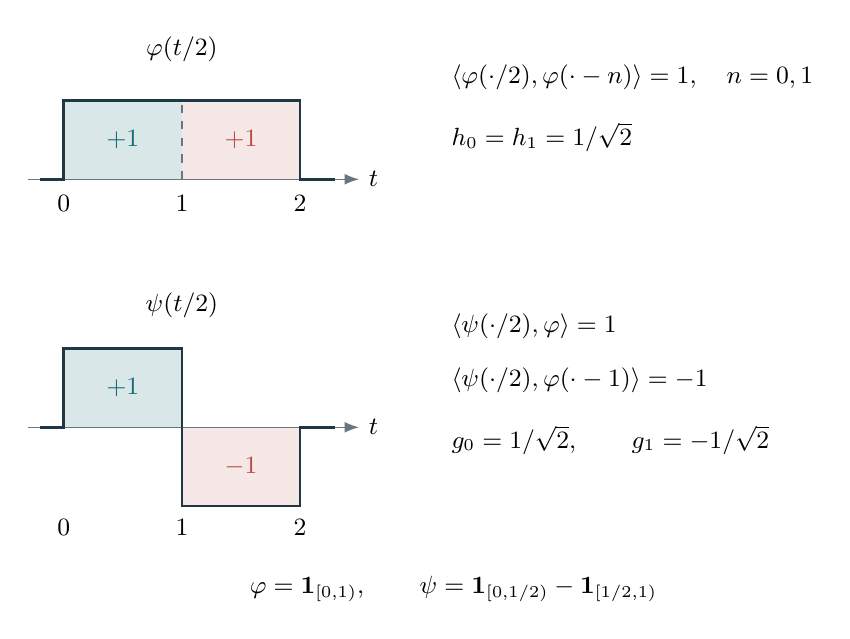
\begin{tikzpicture}[x=1.5cm,y=1cm]
\begin{scope}[shift={(0,2.6)}]
\fill[accent!16] (0,0) rectangle(1,1);\fill[signalred!13] (1,0) rectangle(2,1);
\draw[axis] (-.3,0)--(2.5,0) node[right] {$t$};
\draw[ink,line width=1pt] (-.2,0)--(0,0)--(0,1)--(2,1)--(2,0)--(2.3,0);
\draw[guide] (1,0)--(1,1);
\node at (1,1.65) {$\varphi(t/2)$};
\node[accent] at (.5,.5) {$+1$};\node[signalred] at (1.5,.5) {$+1$};
\foreach \x in {0,1,2} {\node[below] at (\x,-.08) {$\x$};}
\end{scope}
\begin{scope}[shift={(0,-.55)}]
\fill[accent!16] (0,0) rectangle(1,1);\fill[signalred!13] (1,0) rectangle(2,-1);
\draw[axis] (-.3,0)--(2.5,0) node[right] {$t$};
\draw[ink,line width=1pt] (-.2,0)--(0,0)--(0,1)--(1,1)--(1,-1)--(2,-1)--(2,0)--(2.3,0);
\node at (1,1.55) {$\psi(t/2)$};
\node[accent] at (.5,.5) {$+1$};\node[signalred] at (1.5,-.5) {$-1$};
\foreach \x in {0,1,2} {\node[below,fill=white,inner sep=1pt] at (\x,-1.13) {$\x$};}
\end{scope}
\node[anchor=west,align=left] at (3.2,3.5) {$\langle\varphi(\cdot/2),\varphi(\cdot-n)\rangle=1,\quad n=0,1$\\[4mm]$h_0=h_1=1/\sqrt2$};
\node[anchor=west,align=left] at (3.2,.0) {$\langle\psi(\cdot/2),\varphi\rangle=1$\\[3mm]$\langle\psi(\cdot/2),\varphi(\cdot-1)\rangle=-1$\\[4mm]$g_0=1/\sqrt2,\qquad g_1=-1/\sqrt2$};
\node at (3.3,-2.6) {$\varphi=\mathbf1_{[0,1)},\qquad\psi=\mathbf1_{[0,1/2)}-\mathbf1_{[1/2,1)}$};
\end{tikzpicture}
\end{document}
